\chapter{Design}

\section{Methodology}

\begin{figure}[!h]
    \caption{Tree-Shape}
    \centering
    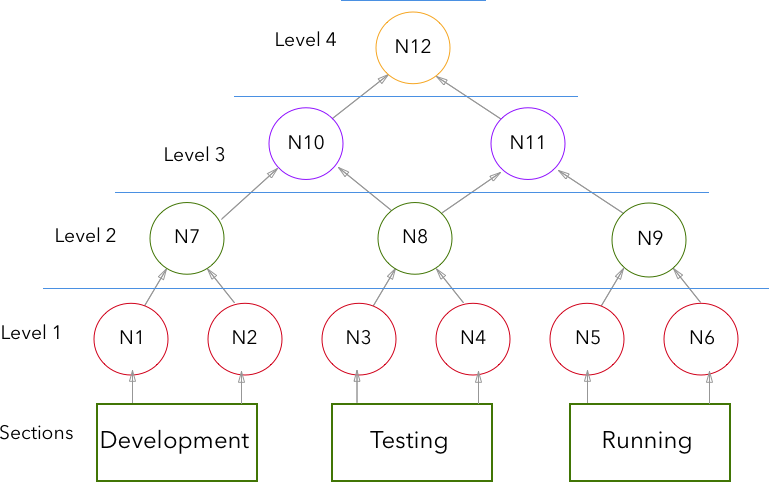
\includegraphics[width=100mm]{images/methodology}
    \label{fig:label}
\end{figure}

% \begin{figure}[!h]
%     \centering
%     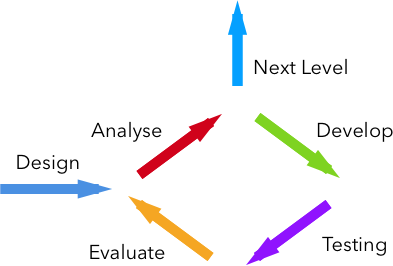
\includegraphics[width=50mm]{images/spiral_model}
%     \label{fig:label}
% \end{figure}

% \begin{figure}[!h]
%     \centering
%     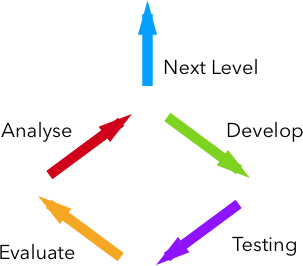
\includegraphics[width=50mm]{images/spiral_model_2}
%     \label{fig:label}
% \end{figure}

After doing research, I decided to implement my own methodology called "Tree-Shaped". The idea behind this methodology is to en-corporate the functionality into different sections, and prove each functionality at a lower, early stage. This benefits by setting out the goal into sections and filling in what functional requirements are need to reach the goal. The proving of functionality part is to able to fix any potential compatibilities at an earlier stage or remove if necessary.

The methodology has three parts

\begin{enumerate}
  \item Sections
  
    The sections stage is first step in using the "tree shaped" methodology. This part is where we set out what we are trying to achieve. Then incorporate each functionality into their respective sections.
    
  \item Functionality   
    
     After we define our sections including their respective functionalities, tests are to be written out for each functionality. This are to show that they still output the correct result, being what they are supposed to do.
    
  \item Levels
  
    Levels stage is where we are proving/testing the functionalists. As we move up the tree into each node, the functionalists are combined together. Thus solving compatibilities issues at an earlier stage of the project development.
\end{enumerate}

\subsection{Advantages}

This methodology is based on the test-driven development (TDD) process that relies on the repetition of very short development cycles. At each level, the nodes which holds the application are tested. These tests are from the functionality part, when combining the previous nodes, we want to make sure they still output the correct result.

\subsection{Disadvantages}

The methodology although sounds good from a theoretical point of view, in a real world it has its drawbacks. Each node (circle in each level) requires making new test application, combing the previous two node applications and potential re-factoring. This takes time where some projects do not have, but we reduce the number of bugs found but re-factoring at each level. To overcome this, the methodology allows to skip one level to reduce testing times.

\section{Functional Requirements}

Functional requirement defines a function of a system or its component. After talking to out-sourced developers and researching current systems out there, the following table \ref{tb:functional} defines the list of functional requirement. They are grouped into sections, what the aim of the project is. 

\begin{table}[h]
\centering
\caption{Functional Requirements}
\label{tb:functional}
\begin{tabular}{|l|l|l|l|l|}
\hline
\cellcolor{green!20}ID & \cellcolor{green!20}Section  & \cellcolor{green!20}Name  & \cellcolor{green!20}Description        & \cellcolor{green!20}Priority \\ \hline
1                      & Development                  & Database storage          & Create, Read, Update, Delete objects   & High   \\ \hline
2                      & Development                  & Push notifications        & Send push notifications to devices     & Medium \\ \hline
3                      & Running                      & Analytics                 & Measure users in app activities        & High   \\ \hline
4                      & Running                      & Backup                    & Backup database to remote site         & Low    \\ \hline
5                      & Running                      & Self hosted               & Host the MBaaS on developers server    & High   \\ \hline
6                      & Running                      & Remote Configuration      & In app live updates                    & High   \\ \hline
7                      & Running                      & A/B Testing               & Testing different variations           & High   \\ \hline
8                      & Development                  & Live Database             & Update objects without user refreshing & Low    \\ \hline
9                      & Development                  & Dashboard                & Interface for developers manage apps   & High   \\ \hline
10                     & Testing                      & Exception catching      & Interface for developers manage apps   & High   \\ \hline
\end{tabular}
\end{table}

\subsection{Development}

\subsubsection{Self hosted}
Allow the developer to host their own system to have full control on when up and running, and not having to worry if the provider is going to shut down the system. By giving the developer a way to host their own back-end then this will keep the cost down of not having to paying for third party services.

\subsubsection{Backup}
This feature gives the developer a piece of mind that the applications data is constantly backup to local or remote location.

\subsubsection{Sprint board}
Challenge faced when creating an application, is trying to keep a list of features or changes to be made for a version. Also knowing history of features already implemented. Their are already different sprint board applications out there, but I wanted a way to en-corporate it all in one single dashboard app, that can be used with teams.


\subsection{Testing}

\subsubsection{Crashes}

\subsection{Running/Live}

\subsubsection{Database}
The API and framework will provide a service to send and retrieve objects to the  database. These tools will not only be able to post and get objects but also to set out filters. Each collection of objects such as users can be viewed in a table format in the dashboard application explained later.

\subsubsection{A/B Testing}
A/B testing also known as split testing is comparing two versions of a page to see which performs better. Currently this popular with web pages but my plan is to bring this to mobile applications. All mobile applications no matter what services they provide all have one goal; a reason to exist. A/B testing allows you to make more out of your existing traffic. This is achieved by sending our to variants ( A and B ) to similar visitors at the same time and use analytics to provide us what version wins. Included in my research, I did a survey to see how end-users respond to different applications. How they look?, Are they concerned on the aesthetics of the app?. At stated end-users do choose whether or not they will continue to use an app. So by using A/B testing service we can quickly find out what they do and do not like. So how can we implement this service in mobile apps? This leads on to my next service.

\subsubsection{Remote Configuration}
Remote configuration is a service that lets you change the behaviour and appearance of the app without requiring the users to download an app update. When using this service, you create the default appearance such as how a button looks, whats the title etc. Then later on we can update this values via the dashboard to configure these. So how does the app know when to get the new version? Included in each request done within the app is the configuration object at the top. This object will tell you, what version is available to download. So why use remote configuration? 
\begin{itemize}
  \item Quickly roll out changes to your app
  \item Customise your app depending on the version they are running
  \item Use this along with A/B testing to find improvements
\end{itemize}

\subsubsection{Notifications}
Allowing the developer to reach their users and perform tasks in the background. These allows the developers to bring the attention of the users to their app if for example a message comes in. A powerful tool to keep the app in real time and the user connected to the app. Ability to add notification certificates relating to each applications and to send individual or bulk notifications.

\subsubsection{Analytics}
Analytics to give the developer real time information on how their app is doing, how users are using their app. Custom tool to configure what data they want to analyse for example, if the applications is based on vehicles then it can be configured to show list of top vehicle type, make or model. Each configuration will have a graph on the main screen. Analytics will also be used for AB Testing service explained later.

\subsection{Non Functional Requirements}

\subsection{Security}
Security is a big part to any cloud based applications. Users personal information being sent up to cloud, where potential hacks could expose these. Not along has able enforcing developers to user HTTPS request, to secure data transmission, I have also taken into account some security measures. 

\subsubsection{Keys}
The systems supports two keys authentication, there is one key that allows requests to access the web server services. The next key allows data back and fourth to the database.

\subsubsection{Database}
Instead of all applications the developer owns being contained in one database, each application created gets their own database. These are only allowed access once the key gets authenticated.


% \section{Project Components}


% % Instead of every application the developer has all being contained in one database, each application created gets their own database. There is one local database which contains the keys for each app. When a request comes in, the main key is authenticated which is stored in a secure file. The second key however is stored in database, when a request to the database is made, the main table is query and the database relating to that 
% % Each application in the dashboard is generated a random sequence of characters, these are to be included in the app builds. 



% \begin{figure}[h]
%     \caption{Framework Overview}
%     \centering
%     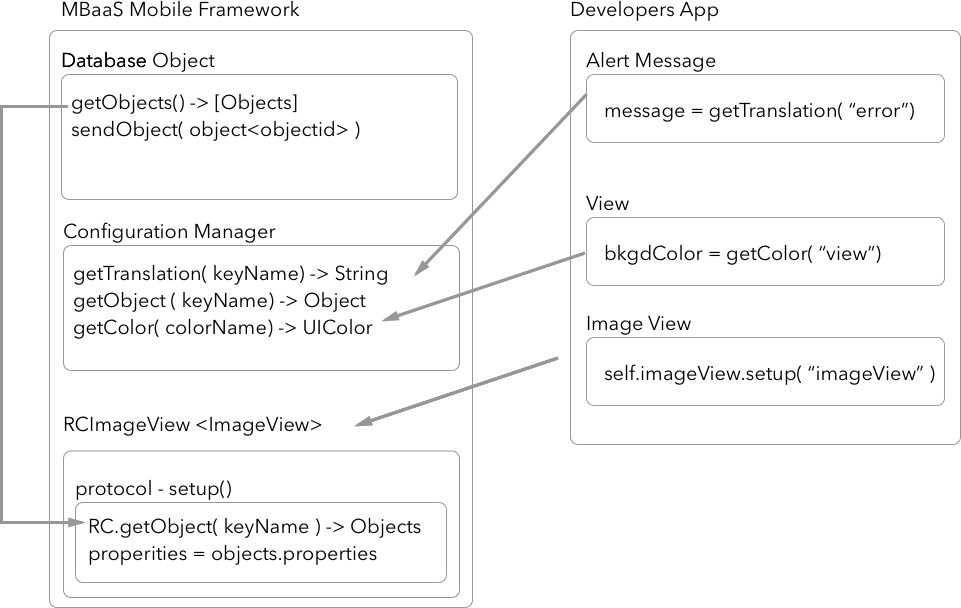
\includegraphics[width=100mm]{images/framwork_architecture}
%     \label{fig:label}
% \end{figure}